\documentclass{article}

\usepackage[margin=1in]{geometry}

\usepackage{lmodern}
\usepackage{amsmath}
\usepackage{amssymb}
\usepackage{upgreek}
\usepackage{pgfplots}
\usepackage[normalem]{ulem}

\pgfplotsset{width=7cm,compat=1.8}
\usetikzlibrary{decorations.markings}


\begin{document}

\section{Curvas Parametrizadas}
De modo geral, podemos descrever uma curva plana por uma \uline{parametriza\c{c}\~ao}:
\[ \vec{r}(t) = (x(t), y(t)) \qquad \text{onde $x(t)$ e $y(t)$ s\~ao fun\c{c}\~oes da vari\'avel $t$.} \]
Exemplo: \\[-5pt]

$y = 2x \quad \rightarrow \quad \vec{r}(t) = (t, 2t)$

\subsection{Vetor Tangente}
O vetor \uline{tangente} \`a curva $\vec{r}(t) = (x(t),\, y(t))$ em um ponto $(x(t_\uplambda),\, y(t_\uplambda))$ \'e:
\[ \vec{v}(t_\uplambda) = \vec{x}\,'(t_\uplambda)\vec{\dot{\imath}} \> + \> \vec{y}\,'(t_\uplambda)\vec{\dot{\jmath}} \]
Denota-se $\vec{r}\,'(t_\uplambda)$. \\[5pt]
Exemplo:

Vetor tangente \`a curva $\vec{r}(t) = (t,\, 2t)$ no ponto $(3, 6)$:
\begin{gather*}
  (3, 6) \>\Rightarrow\> t_\uplambda = 3 \\[5pt]
  \vec{x}\,'(t) = 1 \\
  \vec{y}\,'(t) = 2 \\
  \therefore \\
  \vec{v}\,'(3) = \vec{\dot{\imath}} + 2\vec{\dot{\jmath}}
\end{gather*}
O respectivo vale para curvas no espa\c{c}o.

\subsection{Gr\'aficos}

\begin{tabular}{cc}
  $\vec{r}(t) = (\cos t, 0, \sin t)$ & $\vec{r}(t) = (\cos t, \sin t, t)$ \\[5pt]
  \vtop{\null\hbox{
    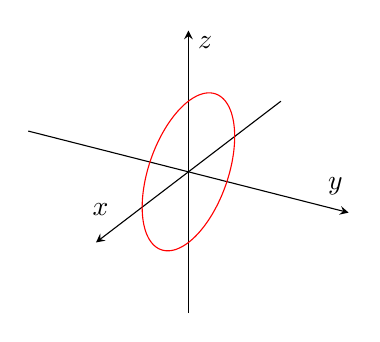
\begin{tikzpicture}
      \begin{axis}[
          view       = {120}{30},
          axis lines = middle,
          xlabel     = $x$,
          ylabel     = $y$,
          zlabel     = $z$,
          zmax       = 2,
          zmin       = -2,
          xmax       = 2,
          xmin       = -2,
          height     = 8cm,
          width      = 8cm,
          xtick      = \empty,
          ytick      = \empty,
          ztick      = \empty
        ]
        \addplot3+ [
          domain    = 0:2*pi,
          samples   = 400,
          samples y = 0,
          mark      = none,
          red,
        ]
        ( {cos(deg(x))}, {0}, {sin(deg(x))} );
      \end{axis}
    \end{tikzpicture}
  }}
  &
  \qquad\vtop{\null\hbox{
    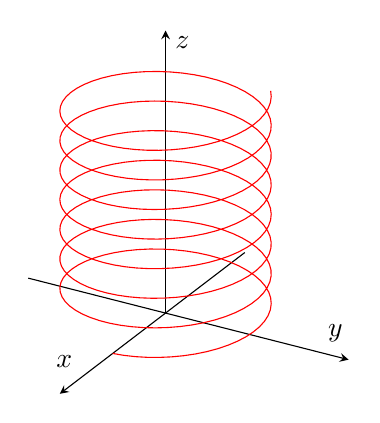
\begin{tikzpicture}
      \begin{axis}[
          view       = {120}{30},
          axis lines = middle,
          xlabel     = $x$,
          ylabel     = $y$,
          zlabel     = $z$,
          zmax       = 60,
          xmax       = 2,
          xmin       = -1.5,
          ymax       = 2,
          ymin       = -1.5,
          height     = 8cm,
          width      = 8cm,
          xtick      = \empty,
          ytick      = \empty,
          ztick      = \empty
        ]
        \addplot3+ [
          domain     = 0:14.7*pi,
          samples    = 400,
          samples y  = 0,
          mark       = none,
          red,
        ]
        ( {cos(deg(x))},{sin(deg(x))},{x});
      \end{axis}
    \end{tikzpicture}
  }}
\end{tabular}

\subsection{Comprimento de Curvas}
\centerline{|graph here|}
Comprimento:
\[ \lim_{\Delta t \to 0} { \sum_i \sqrt{ {\left(\frac{x(t_{i+1}) - x(t)}{\Delta t}\right)}^2 + { \left(\frac {y(t_{i+1}) - y(t)}{\Delta t}\right) }^2 } \cdot \Delta t } = \int\limits_a^b \sqrt{{(x'(t))}^2 + {(y'(t))}^2} \cdot dt \]
\centerline{|example circle here|}



\section{Coordenadas Polares}
\centerline{|graph here|}
\[ P = {(r, \theta)}_{polar} \]

Exemplo: Se $P = {\left(3, \frac{\pi}{4}\right)}_{polar}$ \\
\centerline{|example graph here|}
\underline{Conven\c{c}\~oes}:
\begin{itemize}
  \item $\theta > 0$ se medido, a partir do eixo polar, no sentido anti-hor\'ario.
  \item $\theta < 0$ se medido, a partir do eixo polar, no sentido hor\'ario.
  \item ${(-r, \theta)}_{polar} = {(r, \theta - \pi)}_{polar}$ \\
    \centerline{|example graph here|}
  \item $\forall \theta: {(0, \theta)}_{polar} = 0$
\end{itemize}

\subsection{Rela\c{c}\~ao Entre Sistemas de Coordenadas}
\centerline{|graph here|}
\begin{alignat*}{3}
  &\forall r, \theta &&: {(r, \theta)}_{polar} &&= {(r \cdot \cos \theta,\, r \cdot \sin \theta)}_{ret} \\
  &\forall x, y &&: {(x, y)}_{ret} &&= {\left(\sqrt{x^2 + y^2},\, \arctan{\frac{y}{x}}\right)}_{ret}
\end{alignat*}

\subsection{Curvas Polares}
Uma curva polar \'e definida por uma equa\c{c}\~ao entre as coordenadas polares dos pontos da curva (equa\c{c}\~ao polar). \\

\begin{tabbing}
  Exemplos: \= $r^2 + e^{r\theta} = 0$ \\[5pt]
  \> $0 \cdot \theta + r - 25 = 0 \quad\Rightarrow\quad r = 25$ \\
  \centerline{|circle graph here|}\\[5pt]
  \> $\theta + \frac{\pi}{6} = 0 \quad\Rightarrow\quad \theta = -\frac{\pi}{6}$ \\
  \centerline{|line graph here|}\\[5pt]
  \> $r = \cos{(2\theta)}$ \\[5pt]
  \>\quad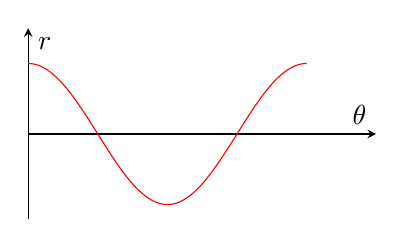
\begin{tikzpicture}
      \begin{axis}[
          axis lines = middle,
          xlabel     = $\theta$,
          ylabel     = $r$,
          xmax       = 3*pi,
          xmin       = pi/2,
          ymax       = 1.5,
          ymin       = -1.2,
          height     = 4cm,
          width      = 6cm,
          xtick      = \empty,
          ytick      = \empty,
        ]
        \addplot [
          domain=0:5*pi/2,
          samples=200,
          red
        ] {sin(deg(x))};
      \end{axis}
    \end{tikzpicture}
\end{tabbing}



\end{document}
